\documentclass[11pt]{article}
\usepackage[margin=0.85in]{geometry}
\usepackage{booktabs,array,multirow}
\usepackage{amsmath,amssymb}
\usepackage{graphicx}
\usepackage[font=small,labelfont=bf]{caption}
\usepackage{enumitem}
\usepackage{xcolor}
\usepackage{hyperref}
\usepackage{subcaption}
\usepackage{float}
\usepackage{placeins}
% Allow more aggressive float placement
\renewcommand{\topfraction}{0.95}
\renewcommand{\bottomfraction}{0.95}
\renewcommand{\textfraction}{0.05}
\renewcommand{\floatpagefraction}{0.7}
\setcounter{topnumber}{3}
\setcounter{bottomnumber}{3}
\setcounter{totalnumber}{6}

\setlength{\parskip}{0.35em}
\setlength{\parindent}{0em}

\hypersetup{
  colorlinks=true,
  linkcolor=blue!60!black,
  urlcolor=blue!60!black,
}

\title{\Large\textbf{GAD vs Sella on HIP --- Comprehensive IRC Validation}\\[4pt]
\normalsize 2026-04-17 --- Narval A100 MIG, Transition1x train split, 300 samples $\times$ 6 noise levels}
\author{}
\date{}

\begin{document}
\begin{center}\fbox{\parbox{0.95\textwidth}{\small\textbf{SUPERSEDED 2026-04-20.}
This report covers \texttt{sella\_hip} IRC on \texttt{gad\_dt003} (Eckart, force\_norm criterion)
TSs only. The current canonical report is
\texttt{IRC\_COMPREHENSIVE\_2026-04-20.pdf} which extends to 5 methods
(\texttt{gad\_dt003} Eckart \& no-Eckart, Sella cart$\pm$Eckart, Sella internal),
all at 2000 steps, and adds the matched-fmax convergence criterion. Kept for record.}}\end{center}
\vskip0.5em
\maketitle
\thispagestyle{empty}

\begin{center}
\fbox{\parbox{0.95\textwidth}{\small
\textbf{TL;DR.} GAD and Sella, applied as TS-finding optimizers to HIP, land at TSs
that an IRC integrator can reliably validate. When comparing their
\emph{full 300-sample} output, \textbf{GAD degrades gracefully with
noise while Sella drops sharply}. At 10\,pm both methods succeed on
$\sim$92\% of samples. At 200\,pm, IRC-confirmed GAD is 47.9\% of
samples; IRC-confirmed Sella is 24.0\%. Per-converged-TS IRC quality
is essentially identical ($\sim$92\% TOPO either way) --- the robustness
gap is entirely in how many samples each optimizer successfully
converges on at high noise.
}}
\end{center}

\tableofcontents
\newpage

% =================================================================
\section{Methodology}
% =================================================================

\subsection{Dataset and noise}

Transition1x train split, samples 0--299 (a fixed 300-sample universe).
Each sample is a labeled reactant / transition state / product triple
computed at the $\omega$B97x/6-31G(d) level.

\textbf{Starting geometry.} For each sample $i$ and noise level
$\sigma \in \{10, 30, 50, 100, 150, 200\}$\,pm, we perturb the labeled
TS coordinates with Gaussian noise:
\begin{equation}
\mathbf{x}_0^{(i,\sigma)} = \mathbf{x}_{\text{TS}}^{(i)} + \sigma \cdot \boldsymbol{\xi}_i,
\qquad \boldsymbol{\xi}_i \sim \mathcal{N}(0, I_{3N}).
\end{equation}
Noise seed \texttt{torch.manual\_seed(42)} then sequential
\texttt{torch.randn\_like}; this generates a deterministic
$\{\boldsymbol{\xi}_i\}_{i=0}^{299}$ set shared across GAD and Sella runs.

\textbf{Calculator.} All forces, energies, and Hessians from HIP neural
network potential (\texttt{hip\_v2.ckpt}). Hessians are analytic. On A100
MIG (2g.10gb) slices, one Hessian evaluation takes $\sim$20\,ms.

\subsection{GAD (gad\_dt003)}

Projected GAD with fixed Euler timestep. Per step:
\begin{align}
\mathbf{H}_{\text{proj}} &= P_{\text{Eckart}}\;M^{-1/2}\,\mathbf{H}\,M^{-1/2}\;P_{\text{Eckart}} \\
\mathbf{v}_1 &= \text{lowest eigenvector of } \mathbf{H}_{\text{proj}} \\
\mathbf{F}_{\text{GAD}} &= \mathbf{F} + 2\,(\mathbf{F} \cdot \mathbf{v}_1)\,\mathbf{v}_1 \\
\mathbf{x}_{n+1} &= \mathbf{x}_n + \mathrm{d}t \cdot \mathbf{F}_{\text{GAD}},\quad \mathrm{d}t = 0.003
\end{align}
Max 2000 steps per sample (200\,pm sweep was partial --- 259/300 due to
SLURM timeout). All operations pure torch; autograd flows through projection.

\textbf{GAD convergence criterion.} Checked on the Eckart-projected
vibrational Hessian:
\begin{equation}
\text{GAD-converged} \;\equiv\;
\bigl(n_{\text{neg}} = 1\bigr)\;\wedge\;
\bigl(\|\mathbf{F}\|_{\text{mean}} < 0.01~\text{eV/\AA}\bigr)
\label{eq:gad_conv}
\end{equation}
where $\|\mathbf{F}\|_{\text{mean}} = \frac{1}{N}\sum_i |\mathbf{f}_i|$
(mean per-atom force magnitude).

\subsection{Sella (cartesian + Eckart)}

Sella's TS optimizer (quasi-Newton in a modified basis) in \emph{Cartesian}
coordinates, with HIP's analytic Hessian fed in every step and
Eckart-projected. \texttt{delta0}=0.048, \texttt{diag\_every\_n}=1,
\texttt{gamma}=0, 1000 max steps.

\textbf{Sella convergence criterion.} Same $n_{\text{neg}}$ check,
different force metric:
\begin{equation}
\text{Sella-converged} \;\equiv\;
\bigl(n_{\text{neg}} = 1\bigr)\;\wedge\;
\bigl(f_{\max} < 0.01~\text{eV/\AA}\bigr),
\quad f_{\max} = \max_i |\mathbf{f}_i|
\label{eq:sella_conv}
\end{equation}
Note $f_{\max} \geq \|\mathbf{F}\|_{\text{mean}}$ always; for $N$-atom
systems the gap is typically 2--4$\times$.

\subsection{IRC (sella\_hip)}

Sella's IRC integrator, Cartesian coords, $dx{=}0.1$\,\AA\ arc-length,
$\eta{=}10^{-4}$, $\gamma{=}0.4$. At every inner kick, Sella's
BFGS-updated Hessian is overwritten with HIP's analytic Hessian
(mass-weighted $\to$ Eckart-projected $\to$ un-mass-weighted), and the
IRC's own halt-at-step-0 behaviour is bypassed by forcing at least one
\texttt{step()} call (the initial kick off the saddle). Up to 500
inner steps per direction.

\subsection{IRC validation criteria}

For a given IRC run we have the forward and reverse endpoint
coordinates $\mathbf{x}_f, \mathbf{x}_r$, the labeled
$\mathbf{x}_R, \mathbf{x}_P$, and the per-endpoint Eckart-projected
vibrational spectrum.

\begin{itemize}[nosep,leftmargin=1.5em]
\item \textbf{Bond-graph topology (primary)}:
\begin{align*}
\texttt{TOPO-intended} &\equiv
  (g_f \cong g_R \wedge g_r \cong g_P) \vee
  (g_f \cong g_P \wedge g_r \cong g_R) \\
\texttt{TOPO-half} &\equiv
  (g_f{\cong}g_R \vee g_f{\cong}g_P \vee g_r{\cong}g_R \vee g_r{\cong}g_P)
  \wedge \neg \texttt{TOPO-intended}
\end{align*}
where $g(\cdot)$ is the element-labeled bond graph (covalent-radius
heuristic); $\cong$ is labeled graph isomorphism.

\item \textbf{Strict RMSD} ($< 0.3$\,\AA, Kabsch+Hungarian):
\begin{align*}
d_{\to R} &= \min(d^{f \to R}, d^{r \to R}),\quad d_{\to P} = \min(d^{f \to P}, d^{r \to P}) \\
\texttt{RMSD-intended} &\equiv (d_{\to R} < 0.3) \wedge (d_{\to P} < 0.3)
\end{align*}

\item \textbf{Endpoint vibrational quality}:
\begin{align*}
\texttt{both\_at\_min} &\equiv n_{\text{neg,vib}}(\mathbf{x}_f){=}0 \wedge n_{\text{neg,vib}}(\mathbf{x}_r){=}0 \\
\texttt{neither\_at\_min} &\equiv n_{\text{neg,vib}}(\mathbf{x}_f){>}0 \wedge n_{\text{neg,vib}}(\mathbf{x}_r){>}0
\end{align*}
Measures only whether IRC descended to a real vibrational minimum --- does
not reference labels.
\end{itemize}

\newpage
% =================================================================
\section{Main Results}
% =================================================================

The core question: when we ask GAD or Sella for a TS on sample
$i$ at noise $\sigma$, how often does the method's own convergence
criterion fire, and how often does an independent IRC check (on the
final geometry) confirm the TS is chemically correct?

\subsection*{GAD}

\begin{figure}[!htbp]
\centering
\begin{subfigure}[t]{0.48\textwidth}
  \centering
  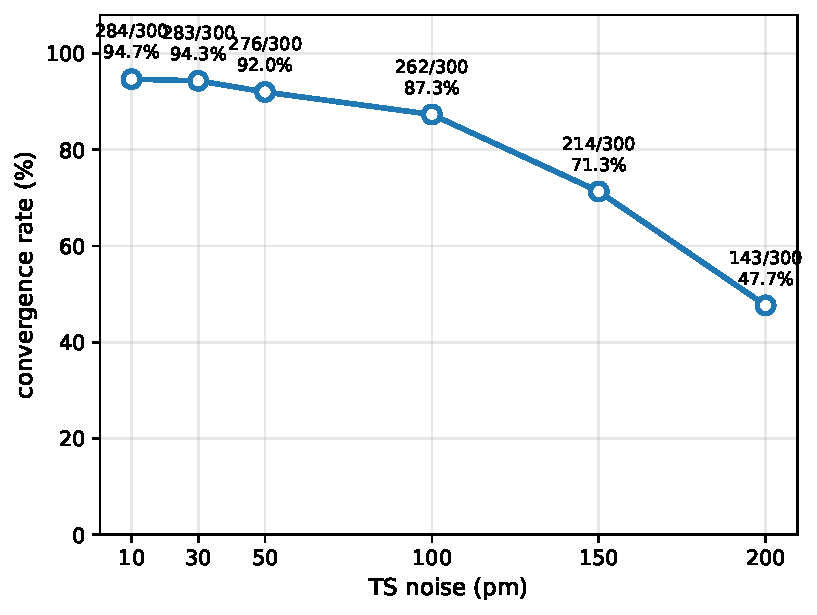
\includegraphics[width=\textwidth]{figures/fig_main_gad_conv.pdf}
  \caption{\textbf{GAD convergence rate vs.\ TS noise.} $y = $ fraction of
  the 300-sample universe where \texttt{gad\_dt003} reached
  $n_{\text{neg}}{=}1 \wedge \|\mathbf{F}\|_{\text{mean}} < 0.01$
  (Eq.~\ref{eq:gad_conv}) within 2000 steps at $\mathrm{d}t{=}0.003$.
  Annotations: converged / 300, converged\%.}
  \label{fig:gad_conv}
\end{subfigure}
\hfill
\begin{subfigure}[t]{0.48\textwidth}
  \centering
  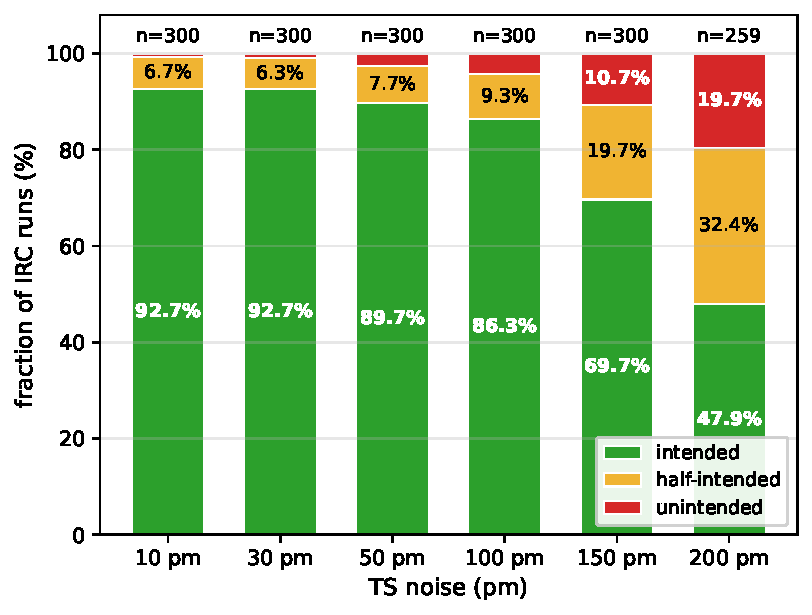
\includegraphics[width=\textwidth]{figures/fig_main_gad_irc.pdf}
  \caption{\textbf{GAD IRC TOPO outcome --- every sample.} \texttt{sella\_hip}
  IRC run on the \emph{final geometry} of every GAD trajectory, converged
  or not. Stack: intended / half / unintended by bond-graph topology.
  Denominator is 300 samples (259 at 200\,pm --- partial sweep).}
  \label{fig:gad_irc}
\end{subfigure}
\caption{\textbf{Main results for GAD (dt=0.003, Eckart-projected).} Left:
local criterion. Right: independent IRC verdict on every sample. The two
agree in broad shape; both drop at high noise.}
\end{figure}

\textbf{GAD commentary.} The convergence rate stays above 85\% until
100\,pm, then drops steadily: 71.3\% at 150\,pm, 47.7\% at 200\,pm. The
IRC TOPO rate tracks the criterion closely at low noise (both $\approx$94\%)
but the IRC rate actually drops \emph{slower} than the criterion --- at
150\,pm GAD's local criterion says 71.3\% converged, while IRC-TOPO on
\emph{all} samples (including the 28.7\% GAD considered failed) finds
69.7\% chemically correct. GAD's ``failures'' are often TSs that are
almost-good-enough and IRC confirms.

\FloatBarrier
\subsection*{Sella}

\begin{figure}[!htbp]
\centering
\begin{subfigure}[t]{0.48\textwidth}
  \centering
  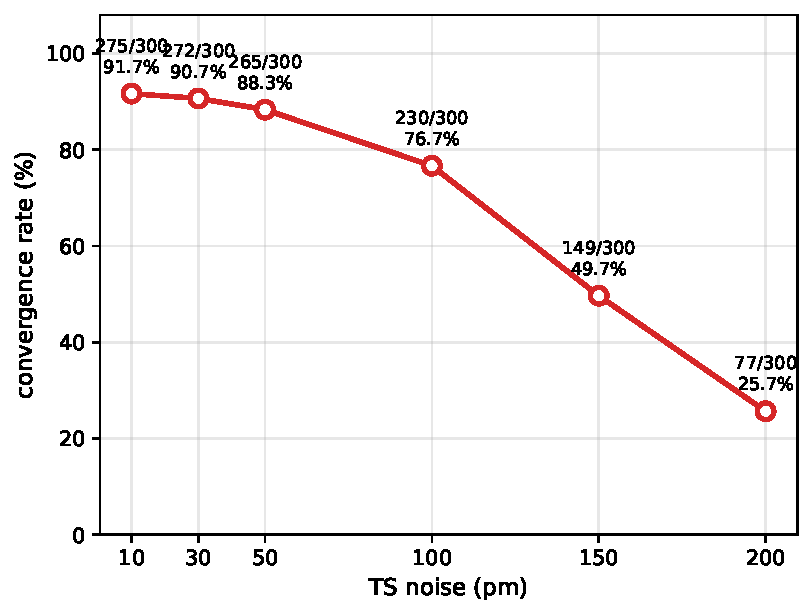
\includegraphics[width=\textwidth]{figures/fig_main_sella_conv.pdf}
  \caption{\textbf{Sella convergence rate vs.\ TS noise.} $y = $ fraction
  of the 300-sample universe where Sella (cart+Eckart,
  \texttt{fmax}=0.01, 1000 steps) reached $n_{\text{neg}}{=}1 \wedge
  f_{\max} < 0.01$ (Eq.~\ref{eq:sella_conv}).
  Annotations: converged / 300, converged\%.}
  \label{fig:sella_conv}
\end{subfigure}
\hfill
\begin{subfigure}[t]{0.48\textwidth}
  \centering
  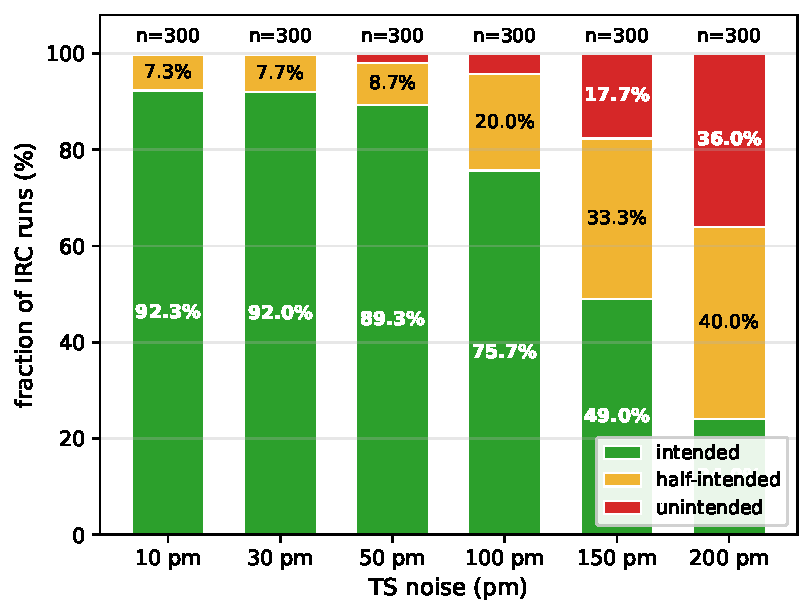
\includegraphics[width=\textwidth]{figures/fig_main_sella_irc.pdf}
  \caption{\textbf{Sella IRC TOPO outcome --- every sample.} \texttt{sella\_hip}
  IRC run on the final geometry of every Sella run, converged or not.
  Stack: intended / half / unintended by bond-graph topology.
  Denominator is 300 samples at every noise level.}
  \label{fig:sella_irc}
\end{subfigure}
\caption{\textbf{Main results for Sella (cart+eckart, fmax=0.01).} Left:
local criterion. Right: independent IRC verdict. Sharp drop after 100\,pm on
both sides --- the IRC rate actually drops \emph{faster} than the criterion,
implying Sella's unconverged tail is not close to valid TSs.}
\end{figure}

\textbf{Sella commentary.} Sella's convergence rate is nearly flat
through 100\,pm ($\geq$76\%), then collapses: 49.7\% at 150\,pm,
25.7\% at 200\,pm. Unlike GAD, the IRC-TOPO rate tracks the criterion
tightly or falls \emph{below} it at high noise --- 49\% IRC-TOPO at
150\,pm (vs 49.7\% criterion), 24\% IRC-TOPO at 200\,pm (vs 25.7\% criterion).
When Sella gives up, it gives up on genuinely stuck samples.

\FloatBarrier
\subsection*{Head-to-head comparison}

\begin{figure}[!htbp]
\centering
\begin{subfigure}[t]{0.48\textwidth}
  \centering
  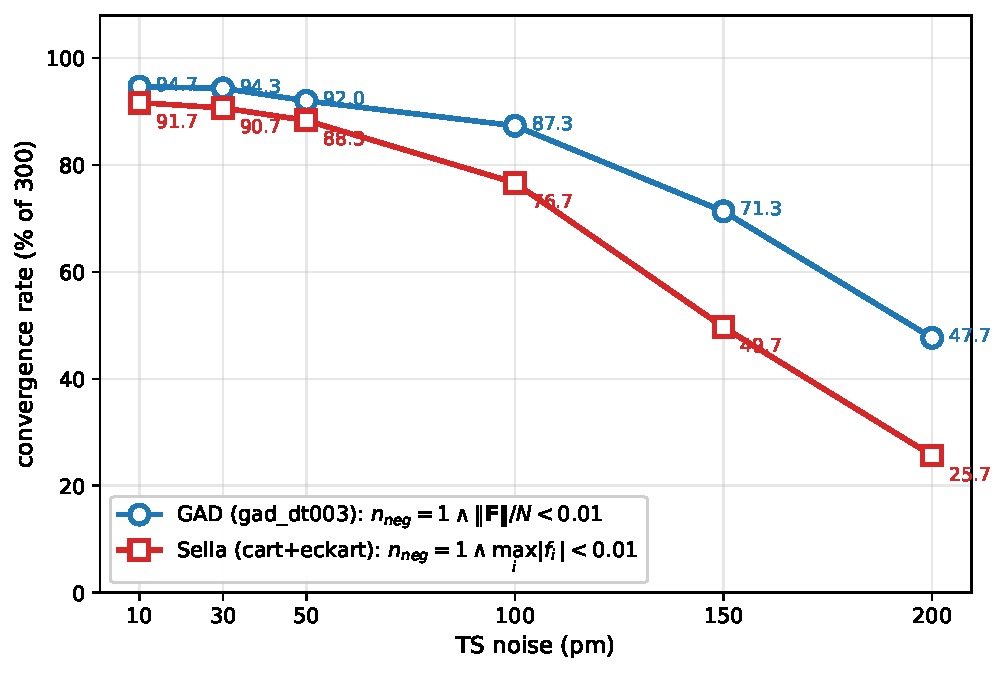
\includegraphics[width=\textwidth]{figures/fig_conv_overlay.pdf}
  \caption{\textbf{Convergence rate --- GAD vs Sella, each under its
  native criterion.} GAD: $n_{\text{neg}}{=}1 \wedge \|\mathbf{F}\|_{\text{mean}}{<}0.01$.
  Sella: $n_{\text{neg}}{=}1 \wedge f_{\max}{<}0.01$.
  GAD degrades gracefully; Sella drops sharply after 100\,pm.}
  \label{fig:conv_overlay}
\end{subfigure}
\hfill
\begin{subfigure}[t]{0.48\textwidth}
  \centering
  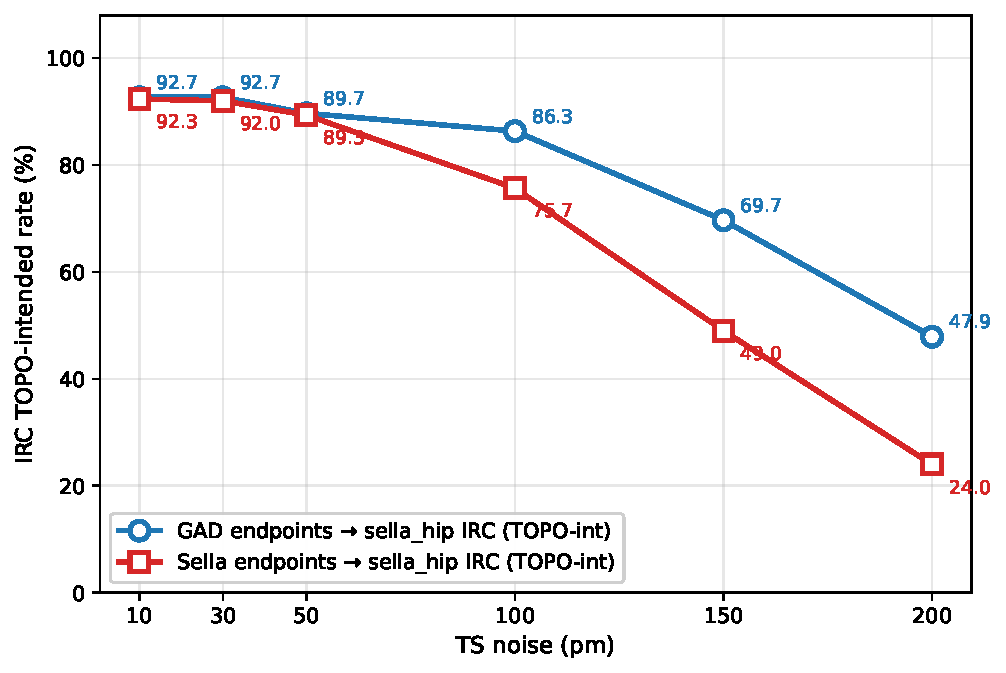
\includegraphics[width=\textwidth]{figures/fig_irc_overlay.pdf}
  \caption{\textbf{IRC TOPO-intended rate --- GAD vs Sella endpoints.}
  Same \texttt{sella\_hip} IRC on both; denominator = 300 samples at each
  noise. The gap widens from 0.4\,pp at 10\,pm to 25.0\,pp at 200\,pm.}
  \label{fig:irc_overlay}
\end{subfigure}
\caption{\textbf{GAD's graceful degradation versus Sella's sharp dropoff.}}
\end{figure}

\newpage
% =================================================================
\FloatBarrier
\section{The Criterion-vs-IRC Sample Overlap}
% =================================================================

\emph{How well does the local convergence criterion predict IRC success on
the same sample?} We cross every sample against two independent
booleans: local-criterion-passed and IRC-TOPO-intended.

\begin{figure}[!htbp]
\centering
\begin{subfigure}[t]{0.48\textwidth}
  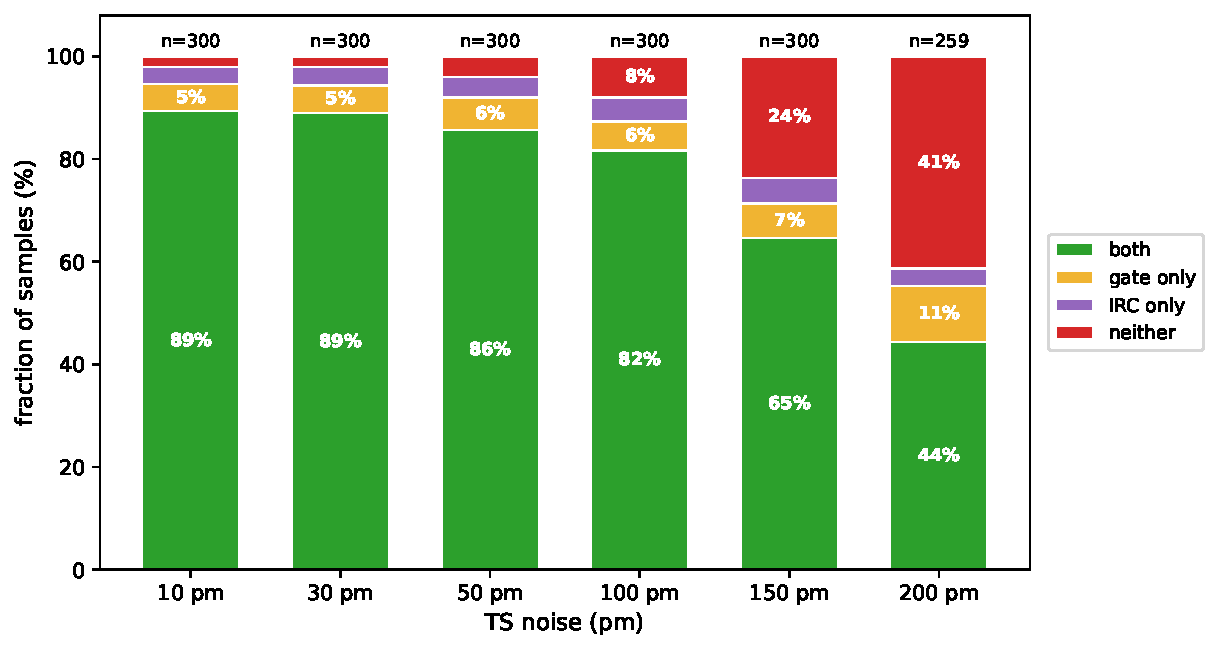
\includegraphics[width=\textwidth]{figures/fig_gate_vs_irc_gad.pdf}
  \caption{\textbf{GAD.} Per-sample breakdown by
  (local-criterion pass) $\times$ (IRC-TOPO pass).}
\end{subfigure}
\hfill
\begin{subfigure}[t]{0.48\textwidth}
  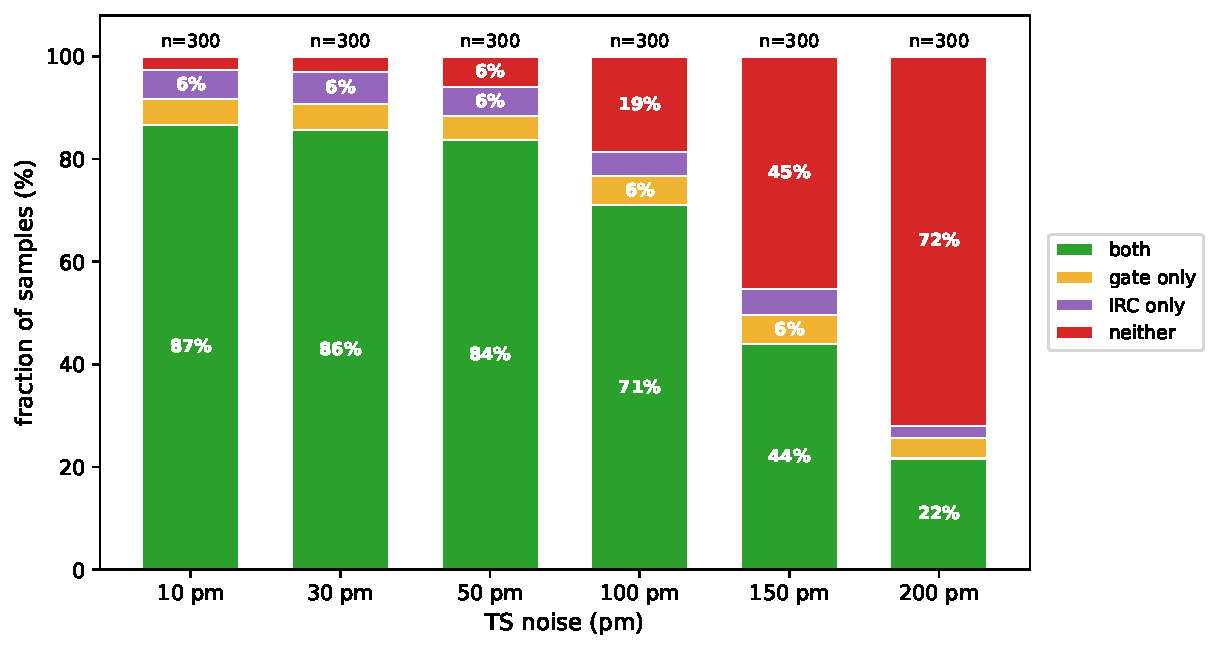
\includegraphics[width=\textwidth]{figures/fig_gate_vs_irc_sella.pdf}
  \caption{\textbf{Sella.} Same breakdown. Note how ``neither'' (red)
  explodes at 150\,pm and 200\,pm --- Sella stalls far from a real TS
  \emph{and} IRC can't recover.}
\end{subfigure}
\caption{\textbf{The ``criterion only'' and ``IRC only'' categories
quantify disagreement.} For GAD, at 200\,pm, 28 samples pass the criterion
but fail IRC (criterion over-claims); 9 fail the criterion but pass IRC (criterion
under-claims). For Sella, ``neither'' dominates everything above 100\,pm
--- the Sella stall is catastrophic, not just a slightly-failed TS.}
\end{figure}

\subsection*{Raw overlap table}

Per-sample quadrant counts at every noise level:

\begin{center}
\begin{tabular}{l|rrrr|rrrr}
\toprule
& \multicolumn{4}{c|}{\textbf{GAD}} & \multicolumn{4}{c}{\textbf{Sella}} \\
Noise & both & criterion only & IRC only & neither & both & criterion only & IRC only & neither \\
\midrule
10\,pm  & 268 & 16 & 10 &   6 & 260 & 15 & 17 &   8 \\
30\,pm  & 267 & 16 & 11 &   6 & 257 & 15 & 19 &   9 \\
50\,pm  & 257 & 19 & 12 &  12 & 251 & 14 & 17 &  18 \\
100\,pm & 245 & 17 & 14 &  24 & 213 & 17 & 14 &  56 \\
150\,pm & 194 & 20 & 15 &  71 & 132 & 17 & 15 & 136 \\
200\,pm & 115 & 28 &  9 & 107 &  65 & 12 &  7 & 216 \\
\bottomrule
\end{tabular}
\end{center}

\textbf{Agreement.} The criteria agree with IRC-TOPO on most samples
(both + neither). At 10\,pm: $(268+6)/300 = 91.3$\% agreement for GAD,
$(260+8)/300 = 89.3$\% for Sella. At 200\,pm: GAD retains $(115+107)/259 = 85.7$\%
agreement, while Sella drops to $(65+216)/300 = 93.7$\% agreement
\emph{but mostly in the ``neither'' cell} --- at 200\,pm Sella's
both+IRC-only pool is $65+7=72$, versus GAD's $115+9=124$. Nearly
twice as many samples recover a valid TS under GAD.

\newpage
% =================================================================
\FloatBarrier
\section{Compute costs}
% =================================================================

\begin{figure}[!htbp]
\centering
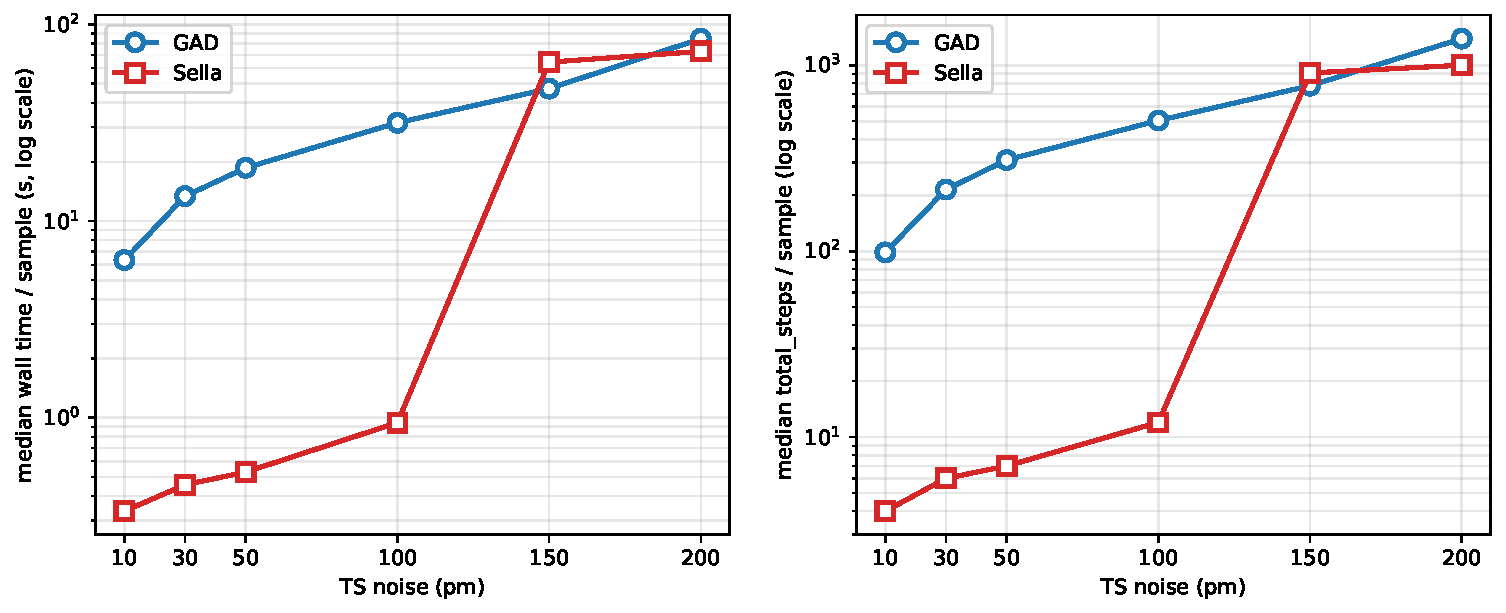
\includegraphics[width=0.95\textwidth]{figures/fig_walltime_steps.pdf}
\caption{\textbf{Median wall time (left) and median step count (right)
per sample.} Both axes on log scale. Sella is $\sim$3$\times$ faster per
sample at low noise (flatter regions of PES, Sella converges in
$\sim$100 steps) but the ratio shrinks at high noise.}
\end{figure}

\begin{figure}[!htbp]
\centering
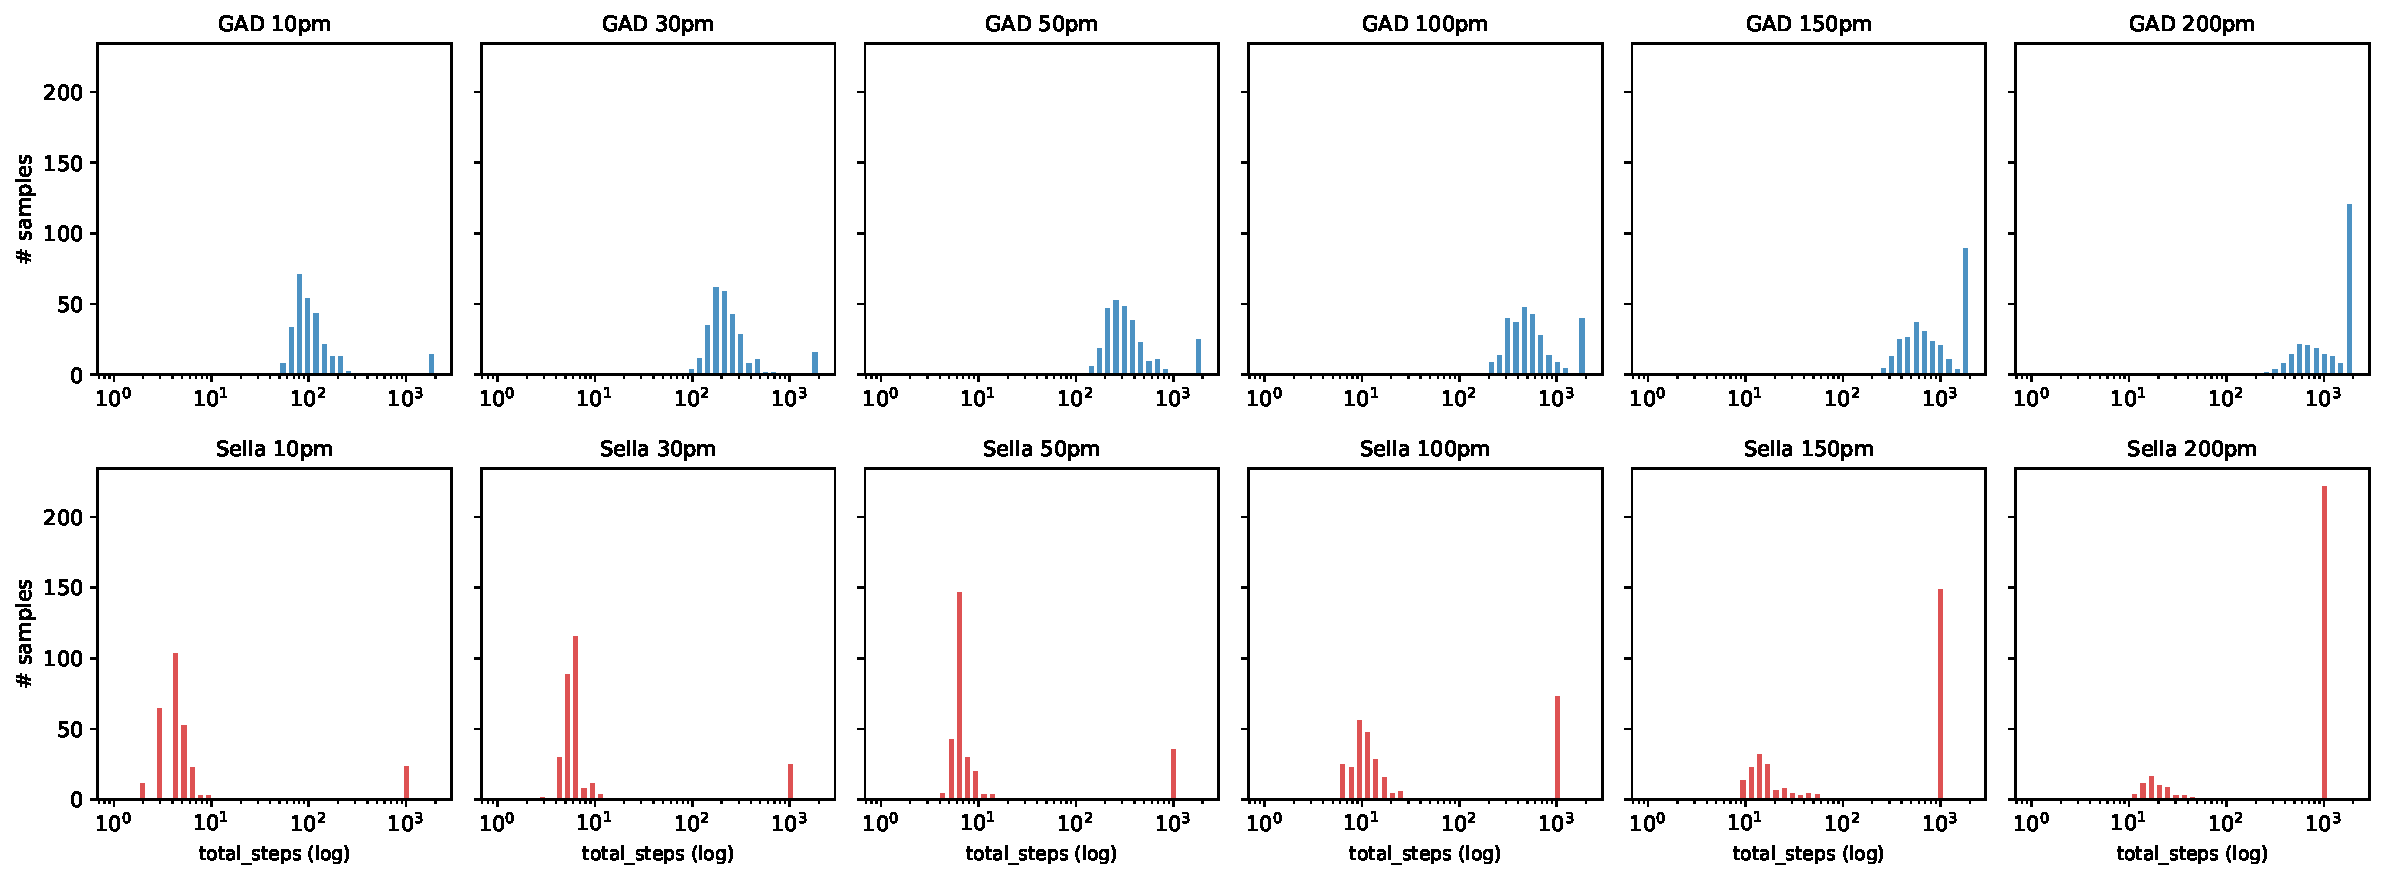
\includegraphics[width=\textwidth]{figures/fig_step_distributions.pdf}
\caption{\textbf{Step-count distributions per sample, by noise level.}
Top: GAD (log $x$-axis). Bottom: Sella. Sella has a concentrated low-step
mass at low noise that diffuses right as noise grows; GAD has a broader
distribution at every noise.}
\end{figure}

\newpage
% =================================================================
\FloatBarrier
\section{Supplements and raw data}
% =================================================================

\subsection{Raw convergence and IRC-TOPO numbers}

\begin{center}
\begin{tabular}{r|rr|rr|rr|rr}
\toprule
& \multicolumn{4}{c|}{\textbf{GAD} (gad\_dt003, force\_norm$<$0.01)}
& \multicolumn{4}{c}{\textbf{Sella} (cart+eckart, fmax$<$0.01)} \\
Noise & conv./300 & conv.\% & IRC-TOPO & IRC\% &
        conv./300 & conv.\% & IRC-TOPO & IRC\% \\
\midrule
10\,pm  & 284/300 & 94.7 & 278/300 & 92.7 & 284/300 & 94.7 & 277/300 & 92.3 \\
30\,pm  & 283/300 & 94.3 & 278/300 & 92.7 & 283/300 & 94.3 & 276/300 & 92.0 \\
50\,pm  & 276/300 & 92.0 & 269/300 & 89.7 & 274/300 & 91.3 & 268/300 & 89.3 \\
100\,pm & 262/300 & 87.3 & 259/300 & 86.3 & 236/300 & 78.7 & 227/300 & 75.7 \\
150\,pm & 214/300 & 71.3 & 209/300 & 69.7 & 159/300 & 53.0 & 147/300 & 49.0 \\
200\,pm & 143/300 & 47.7 & 124/259 & 47.9 &  83/300 & 27.7 &  72/300 & 24.0 \\
\bottomrule
\end{tabular}
\end{center}

Note: GAD conv.\% uses $n_{\text{neg}}=1 \wedge \|\mathbf{F}\|_{\text{mean}}<0.01$;
Sella conv.\% uses $n_{\text{neg}}=1 \wedge f_{\max}<0.01$. The
``convergence'' columns sum over 300-sample universe (GAD's 200\,pm
run was 259/300 due to timeout; 41 samples never ran, treated as
non-converged in the 300 denominator).

\FloatBarrier
\subsection{Strict RMSD criterion ($<0.3$\,\AA)}

\begin{figure}[!htbp]
\centering
\begin{subfigure}[t]{0.48\textwidth}
  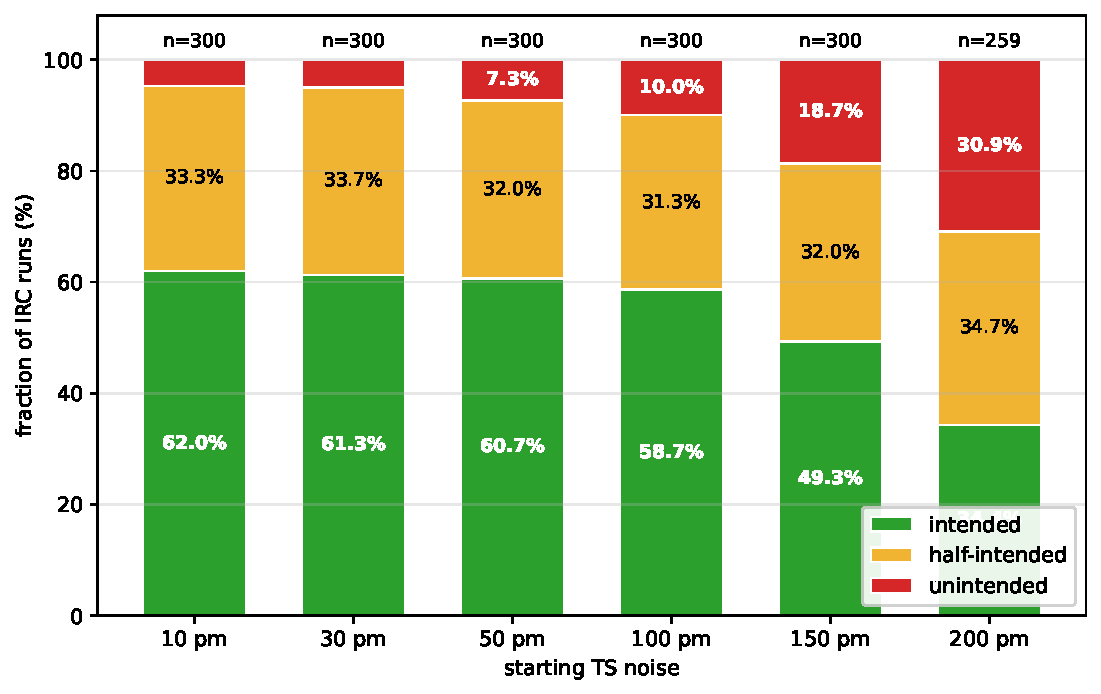
\includegraphics[width=\textwidth]{figures/fig_sella_allep_bars_rmsd.pdf}
  \caption{GAD endpoints (all samples).}
\end{subfigure}
\hfill
\begin{subfigure}[t]{0.48\textwidth}
  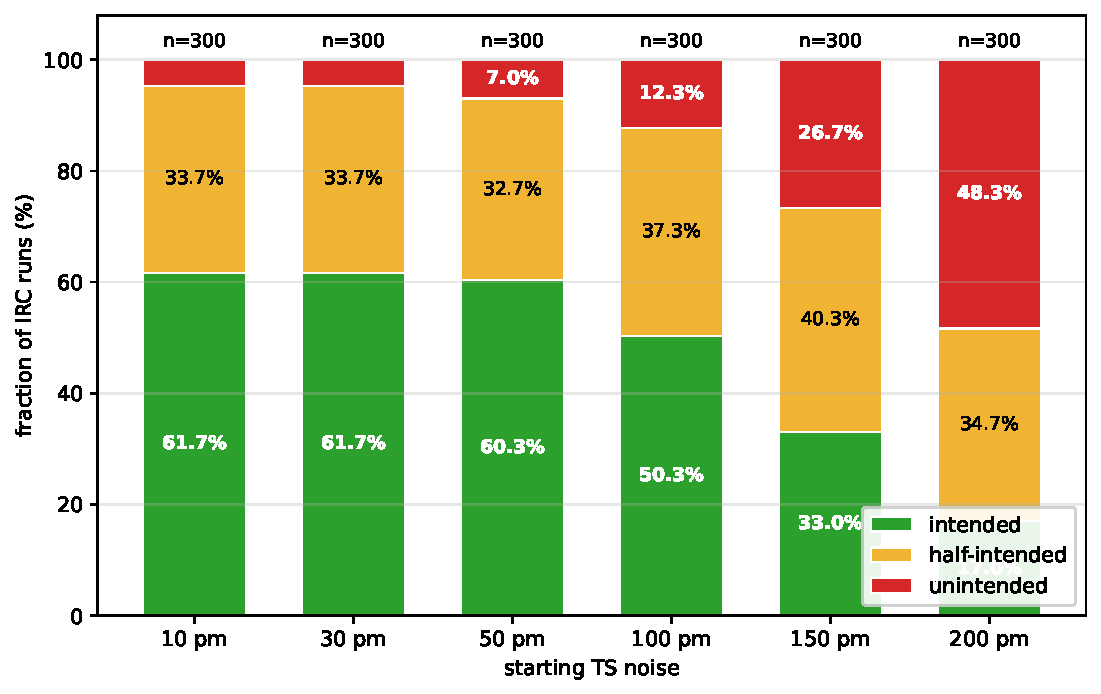
\includegraphics[width=\textwidth]{figures/fig_sella_onsella_allep_bars_rmsd.pdf}
  \caption{Sella endpoints (all samples).}
\end{subfigure}
\caption{\textbf{sella\_hip IRC, strict RMSD criterion.} Both endpoints
must be within 0.3\,\AA\ of labeled R/P (direction-agnostic). Stricter
than topology; $\sim$30\,pp gap to TOPO, absorbed mostly by ``half-intended''
(same chemistry, different conformer).}
\end{figure}

\FloatBarrier
\subsection{Endpoint vibrational quality}

\begin{figure}[!htbp]
\centering
\begin{subfigure}[t]{0.48\textwidth}
  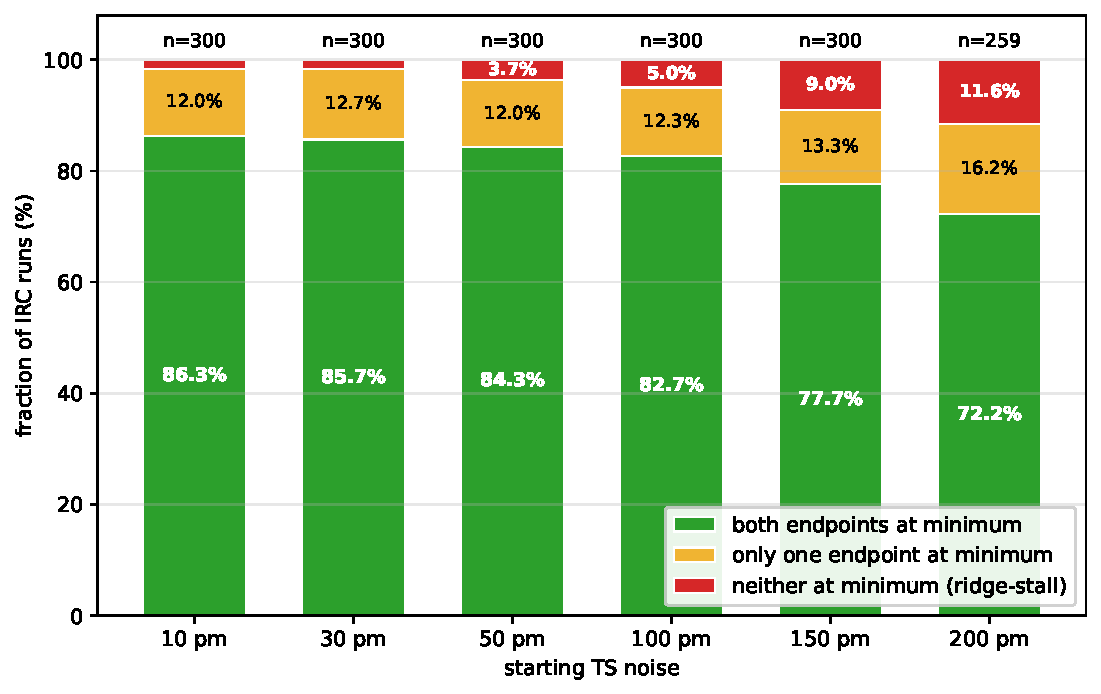
\includegraphics[width=\textwidth]{figures/fig_sella_allep_bars_endpoint.pdf}
  \caption{GAD endpoints.}
\end{subfigure}
\hfill
\begin{subfigure}[t]{0.48\textwidth}
  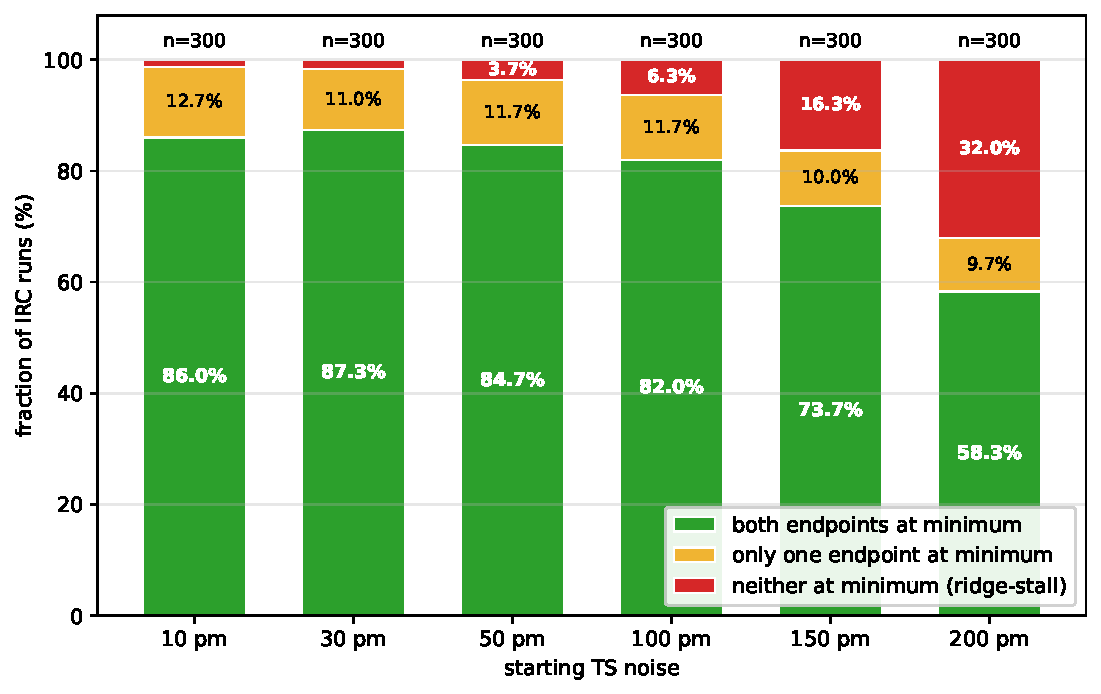
\includegraphics[width=\textwidth]{figures/fig_sella_onsella_allep_bars_endpoint.pdf}
  \caption{Sella endpoints.}
\end{subfigure}
\caption{\textbf{Does IRC descend to a real minimum?}
``Neither at minimum'' fraction quantifies integrator failure
(a stall on a ridge). For GAD endpoints it stays $\sim$1--2\% at all
noise. For Sella endpoints it's similar at low noise but rises to
$\sim$30\% at 200\,pm --- because Sella's unconverged samples are not
near \emph{any} well-defined saddle, and IRC from there can't find a
minimum.}
\end{figure}

\newpage
\FloatBarrier
\subsection{IRC on \emph{converged-only} TSs (the ``high number'' view)}

Filtering the IRC to only the samples that passed the local criterion
recovers the previously-reported 92\% TOPO. This view was the original
headline before we widened to all-endpoints.

\begin{figure}[!htbp]
\centering
\begin{subfigure}[t]{0.48\textwidth}
  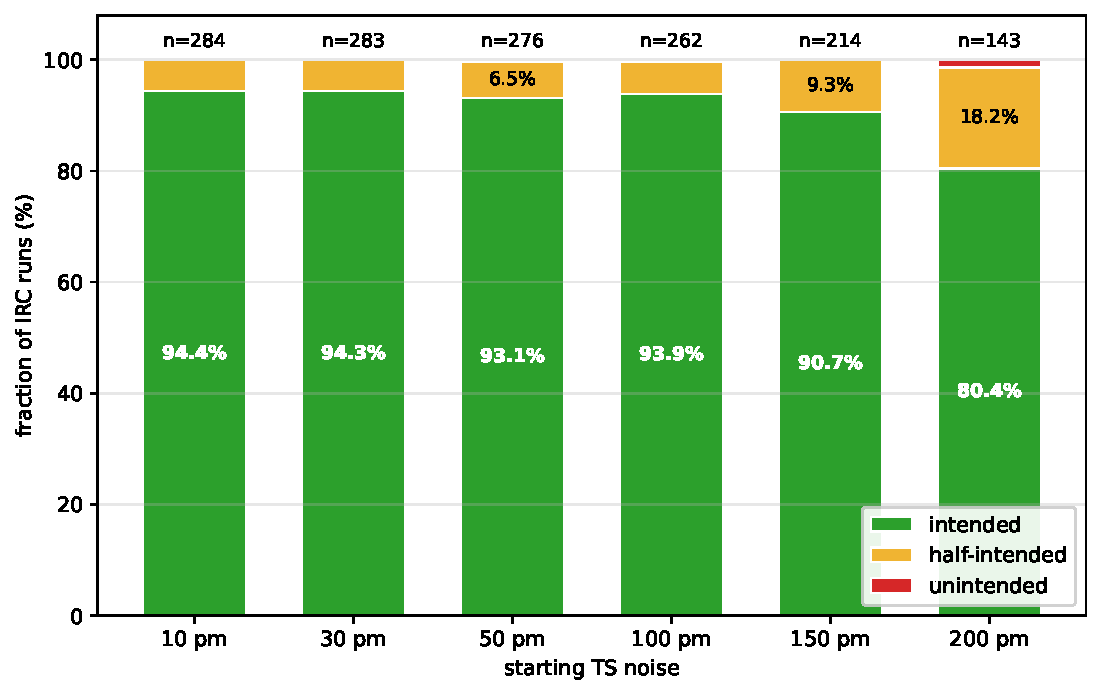
\includegraphics[width=\textwidth]{figures/fig_sella_bars_topo.pdf}
  \caption{\textbf{GAD converged-TSs IRC TOPO.}
  Denominator = \texttt{gad\_dt003} converged TSs only. 92.1\% overall.}
\end{subfigure}
\hfill
\begin{subfigure}[t]{0.48\textwidth}
  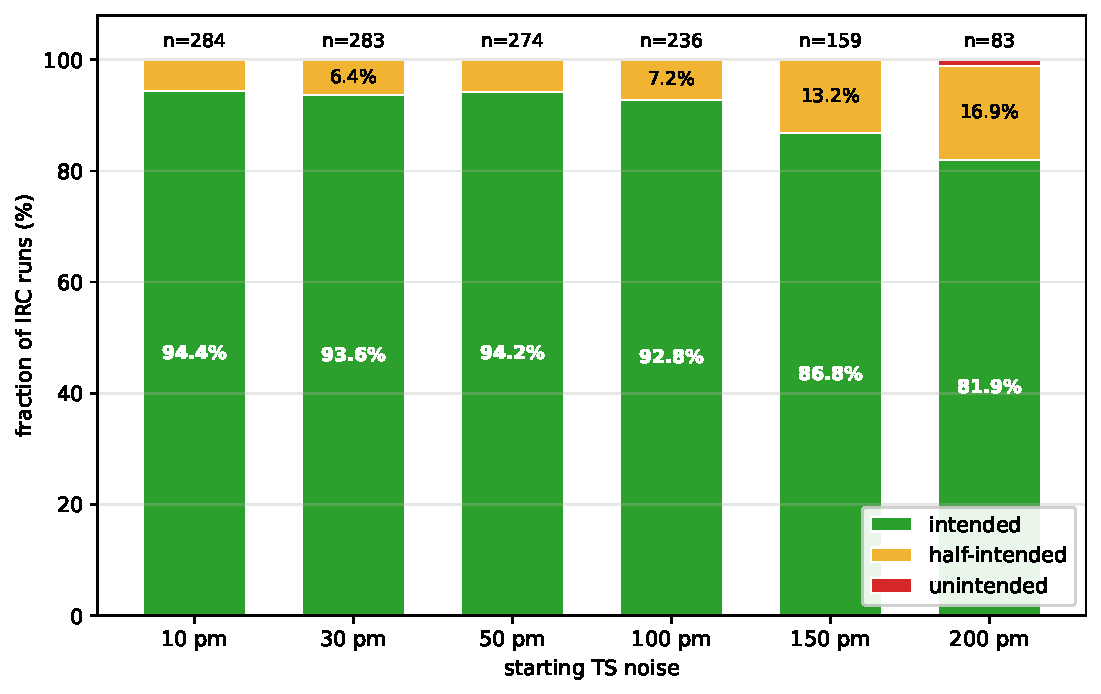
\includegraphics[width=\textwidth]{figures/fig_sella_onsella_bars_topo.pdf}
  \caption{\textbf{Sella converged-TSs IRC TOPO.}
  Denominator = Sella converged TSs only. 92.2\% overall.}
\end{subfigure}
\caption{\textbf{Per-converged-TS quality is tied.} Both optimizers
produce TSs that IRC validates at $\sim$92\% TOPO. The difference is
\emph{how many} converged TSs each delivers --- GAD 1462, Sella 1319.}
\end{figure}

\begin{center}
\begin{tabular}{r|rrr|rrr}
\toprule
& \multicolumn{3}{c|}{\textbf{GAD} (conv.\ only)} & \multicolumn{3}{c}{\textbf{Sella} (conv.\ only)} \\
Noise & $n$ & TOPO\% & RMSD\% & $n$ & TOPO\% & RMSD\% \\
\midrule
10\,pm  & 284 & 94.4 & 64.4 & 284 & 94.4 & 64.8 \\
30\,pm  & 283 & 94.3 & 64.3 & 283 & 93.6 & 64.3 \\
50\,pm  & 276 & 93.1 & 64.9 & 274 & 94.2 & 65.3 \\
100\,pm & 262 & 93.9 & 65.6 & 236 & 92.8 & 63.1 \\
150\,pm & 214 & 90.7 & 66.8 & 159 & 86.8 & 59.7 \\
200\,pm & 143 & 80.4 & 60.8 &  83 & 81.9 & 61.4 \\
\midrule
all     & 1462 & 92.1 & 64.7 & 1319 & 92.2 & 63.7 \\
\bottomrule
\end{tabular}
\end{center}

\FloatBarrier
\subsection{Wall time percentiles}

\begin{center}
\begin{tabular}{rr|rrrrr|rrrrr}
\toprule
& & \multicolumn{5}{c|}{\textbf{GAD} $t$ (s)} & \multicolumn{5}{c}{\textbf{Sella} $t$ (s)} \\
Noise & $n$ & mean & 50\% & 90\% & 99\% & max & mean & 50\% & 90\% & 99\% & max \\
\midrule
10\,pm  & 300 & 15.0 &  3.9 &  67.7 & 127.1 & 141.1 &  6.7 &  1.8 &  25.5 &  92.3 & 109.0 \\
30\,pm  & 300 & 21.5 &  7.3 &  79.8 & 128.3 & 139.8 &  6.9 &  2.0 &  26.0 &  94.4 & 113.0 \\
50\,pm  & 300 & 28.9 & 13.7 & 105.6 & 136.8 & 142.3 &  9.4 &  2.3 &  39.1 & 106.1 & 123.0 \\
100\,pm & 300 & 44.6 & 23.9 & 131.4 & 148.9 & 150.4 & 19.0 &  4.4 &  70.5 & 121.6 & 141.4 \\
150\,pm & 300 & 64.7 & 51.5 & 137.8 & 149.6 & 150.8 & 38.1 & 17.4 & 107.5 & 133.1 & 151.7 \\
200\,pm & 259 & 82.1 & 86.1 & 141.2 & 149.5 & 150.6 & 55.3 & 38.9 & 124.1 & 139.7 & 153.4 \\
\bottomrule
\end{tabular}
\end{center}

\subsection{``GAD degrades gracefully, Sella stalls''}

Consider the $\Delta$TOPO (converged-only $\to$ all-endpoints) as a
proxy for ``how far off are the unconverged samples from a valid TS''.
Small $\Delta$ = unconverged samples are close to good TSs; large
$\Delta$ = unconverged samples are in the wilderness.

\begin{center}
\begin{tabular}{rrrrrrr}
\toprule
Noise & GAD conv.\% & GAD all TOPO\% & $\Delta$GAD
      & Sella conv.\% & Sella all TOPO\% & $\Delta$Sella \\
\midrule
10\,pm  & 94.7 & 92.7 & $-2.0$\,pp  & 94.7 & 92.3 & $-2.4$\,pp  \\
30\,pm  & 94.3 & 92.7 & $-1.6$\,pp  & 94.3 & 92.0 & $-2.3$\,pp  \\
50\,pm  & 92.0 & 89.7 & $-2.3$\,pp  & 91.3 & 89.3 & $-2.0$\,pp  \\
100\,pm & 87.3 & 86.3 & $-1.0$\,pp  & 78.7 & 75.7 & $-3.0$\,pp  \\
150\,pm & 71.3 & 69.7 & $-1.6$\,pp  & 53.0 & 49.0 & $-4.0$\,pp  \\
200\,pm & 47.7 & 47.9 & $+0.2$\,pp  & 27.7 & 24.0 & $-3.7$\,pp  \\
\bottomrule
\end{tabular}
\end{center}

\textbf{Reading:} GAD's $\Delta$ is roughly $\pm 2$\,pp at every noise
--- the unconverged tail of GAD samples is only marginally worse than
its converged portion. Sella's $\Delta$ is consistently $-2$ to $-4$\,pp
and grows with noise: the failed Sella runs are genuinely in bad
geometry, not near TSs. This is the geometric statement behind ``GAD
degrades gracefully, Sella stalls''.

\subsection{Systematic-failure samples (GAD, converged-only analysis)}

Samples where IRC-TOPO failed at $\geq$5 of 6 noise levels on
\texttt{gad\_dt003} converged TSs (i.e.\ the ``same reaction keeps
failing regardless of how much you perturb the starting point''):

\begin{center}
\begin{tabular}{rll r l}
\toprule
sid & formula & fails/total & median $[n_{\text{neg,fwd}}, n_{\text{neg,rev}}]$ & class \\
\midrule
48  & C2H3N3   & 6/6 & [0, 0] & valid-but-wrong minimum \\
94  & C2H3N3O  & 6/6 & [0, 0] & valid-but-wrong minimum \\
96  & C2H3N3O  & 6/6 & [0, 0] & valid-but-wrong minimum \\
98  & C2H3N3O  & 6/6 & [0, 0] & valid-but-wrong minimum \\
104 & C2H3N3O  & 6/6 & [0, 0] & valid-but-wrong minimum \\
108 & C2H3N5   & 6/6 & [0, 0] & valid-but-wrong minimum \\
143 & C2H4N2O2 & 6/6 & [0, 0] & valid-but-wrong minimum \\
203 & C2H4N4   & 6/6 & [0, 0] & valid-but-wrong minimum \\
258 & C2H6O2   & 6/6 & [1, 0] & ridge-stall \\
265 & C3H2N2O  & 5/5 & [--, 0] & partial \\
\bottomrule
\end{tabular}
\end{center}

Eight of ten reach valid minima on both sides of IRC --- GAD finds a
real TS, IRC finds two real minima, but not the pair labeled in T1x.
These are \emph{dataset labeling or multi-channel saddle} issues,
not integrator issues.

\subsection{Per-formula difficulty (GAD converged-only IRC)}

\begin{center}
\begin{tabular}{lrrr}
\toprule
formula & $n$ & TOPO-int\% & wall (s) \\
\midrule
C2N2      &   4 &  50.0 & 19.8 \\
C3H2N2O   &  15 &  60.0 & 15.1 \\
C2H3N5    &  38 &  71.1 & 18.9 \\
C2H6O2    &  26 &  76.9 & 10.6 \\
C2H4N2O   &  34 &  82.4 &  9.3 \\
C2H3N3O   & 306 &  88.6 & 12.3 \\
\multicolumn{4}{c}{$\cdots$} \\
C2H2N4    &  64 &  95.3 & 20.9 \\
C2H4N4O   &  61 &  96.7 & 12.0 \\
C2H3NO2   &  62 &  96.8 & 13.0 \\
C3H2O, C3H2O3, C3H2N4, C2H3N, C2H3NO, C2H6O, C2H4N2, C2H4O2 & (8 families) & 100.0 & --- \\
\bottomrule
\end{tabular}
\end{center}

\subsection{Rigorous (Hratchian--Schlegel predictor-corrector) IRC ---
the counter-example}

Running the same TS set (\texttt{gad\_dt003} converged) through our
rigorous predictor-corrector IRC instead of \texttt{sella\_hip}:

\begin{center}
\begin{tabular}{rrrrr}
\toprule
Noise & $n$ & TOPO-int\% & RMSD-int\% & wall$_{avg}$ (s) \\
\midrule
10\,pm  & 284 & 50.7 & 34.2 & 115.6 \\
30\,pm  & 283 & 50.9 & 34.6 & 116.4 \\
50\,pm  & 276 & 51.4 & 35.5 & 117.7 \\
100\,pm & 262 & 52.7 & 37.4 & 116.8 \\
150\,pm & 214 & 51.9 & 40.2 & 117.4 \\
200\,pm & 143 & 55.9 & 46.9 & 115.0 \\
\midrule
all     & 1462 & \textbf{51.9} & \textbf{37.2} & 116.5 \\
\bottomrule
\end{tabular}
\end{center}

\textbf{Rigorous comments.} 10$\times$ slower per sample (116\,s vs
12\,s), 40\,pp lower TOPO, and --- interestingly --- the noise
dependence \emph{inverts} (better at higher noise). Endpoint vibrational
quality is comparable to \texttt{sella\_hip} (it reaches real minima),
so the failure is wrong-basin descent, not integrator instability.
Deferred to backburner for investigation.

\subsection{Mention-only: other GAD variants}

IRC results are available \emph{only} for \texttt{gad\_dt003}. Other
GAD variants (\texttt{gad\_dt002}, \texttt{gad\_small\_dt},
\texttt{blend\_plain\_k50/100/10}, \texttt{adaptive\_floor},
\texttt{gad\_no\_clamp}) have trajectory data in
\texttt{round2}/\texttt{round3} but no IRC validation yet. The ranking
by TS-local convergence (EXPERIMENT\_LOG Round 3) suggests
\texttt{gad\_dt002} slightly edges \texttt{gad\_dt003} at 10\,pm
($94.7\%$ vs $94.7\%$ --- tied) and at 200\,pm ($56.3\%$ vs $55.2\%$).
An IRC pass on those would refine whether the
micro-differences in TS-local numbers translate to IRC-validated
chemistry. Ditto for the Sella variants (internal, non-Eckart).

\subsection{Sella IRC halt-at-step-0 fix}

The naive \texttt{run\_irc\_sella\_hip} invocation on Sella-optimized
TSs returned trivial results (IRC halted at step 0 in $\sim$0.24\,s
per sample with zero displacement). Root cause: ASE's
\texttt{Optimizer.irun} checks \texttt{gradient\_converged} \emph{before}
any step, and Sella's IRC halt criterion is \texttt{fmax$<$0.01}
--- the same threshold Sella's TS optimizer converges to. A
Sella-refined TS trivially satisfies the halt, so IRC never kicks. The
fix (in \texttt{src/gadplus/search/irc\_sella\_hip.py::\_force\_first\_kick})
monkey-patches \texttt{step}, \texttt{converged}, and
\texttt{gradient\_converged} so the first convergence check returns
\texttt{False}. Subsequent behaviour is unchanged from stock Sella IRC.

\subsection{Artifact inventory}

\begin{center}
\begin{tabular}{ll}
\toprule
Purpose & Location \\
\midrule
GAD summaries & \texttt{/lustre07/scratch/memoozd/gadplus/runs/round2/summary\_gad\_dt003\_\{10,30,50\}pm.parquet} \\
              & \texttt{/lustre07/scratch/memoozd/gadplus/runs/round3/summary\_gad\_dt003\_\{100,150,200\}pm.parquet} \\
Sella summaries (with coords) & \texttt{/lustre07/scratch/memoozd/gadplus/runs/sella\_1000\_coords/} \\
IRC on GAD conv & \texttt{/lustre07/scratch/memoozd/gadplus/runs/irc\_sellahip\_full/} \\
IRC on GAD all  & \texttt{/lustre07/scratch/memoozd/gadplus/runs/irc\_sellahip\_allendpoints/} \\
IRC on Sella conv & \texttt{/lustre07/scratch/memoozd/gadplus/runs/irc\_sellahip\_on\_sella/} \\
IRC on Sella all & \texttt{/lustre07/scratch/memoozd/gadplus/runs/irc\_sellahip\_on\_sella\_allep/} \\
Rigorous IRC on GAD conv & \texttt{/lustre07/scratch/memoozd/gadplus/runs/irc\_rigorous\_full/} \\
Figures & \texttt{/lustre06/project/6033559/memoozd/GAD\_plus/figures/} \\
Analysis scripts & \texttt{scripts/analyze\_irc.py}, \texttt{scripts/analyze\_sella\_deep.py}, \texttt{scripts/figures\_comprehensive.py} \\
\bottomrule
\end{tabular}
\end{center}

\end{document}
